\documentclass{article}
\usepackage{tikz}

\begin{document}

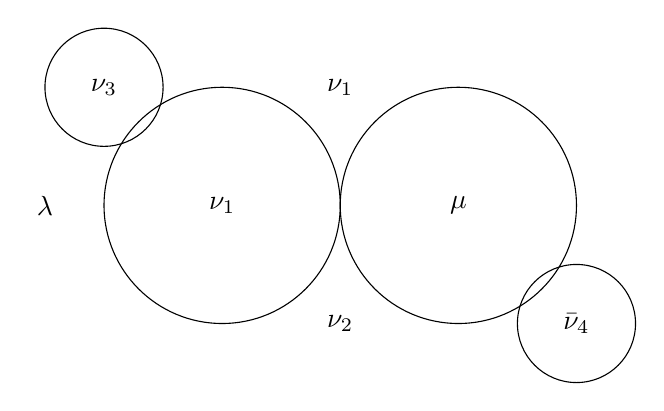
\begin{tikzpicture}[scale=1.5]
    % Draw the circles
    \draw (0,0) circle (1);
    \draw (2,0) circle (1);
    \draw (-1,1) circle (0.5);
    \draw (3,-1) circle (0.5);
    
    % Label the circles
    \node at (0,0) {$\nu_1$};
    \node at (2,0) {$\mu$};
    \node at (-1,1) {$\nu_3$};
    \node at (3,-1) {$\bar{\nu}_4$};
    \node at (-1.5,0) {$\lambda$};
    \node at (1,-1) {$\nu_2$};
    \node at (1,1) {$\nu_1$};
\end{tikzpicture}

\end{document}